\documentclass{standalone}
\usepackage{tikz}
\usetikzlibrary{patterns, positioning}
\usepackage[sfdefault]{ClearSans} %% option 'sfdefault' activates Clear Sans as the default text font
\usepackage[T1]{fontenc}

\begin{document}
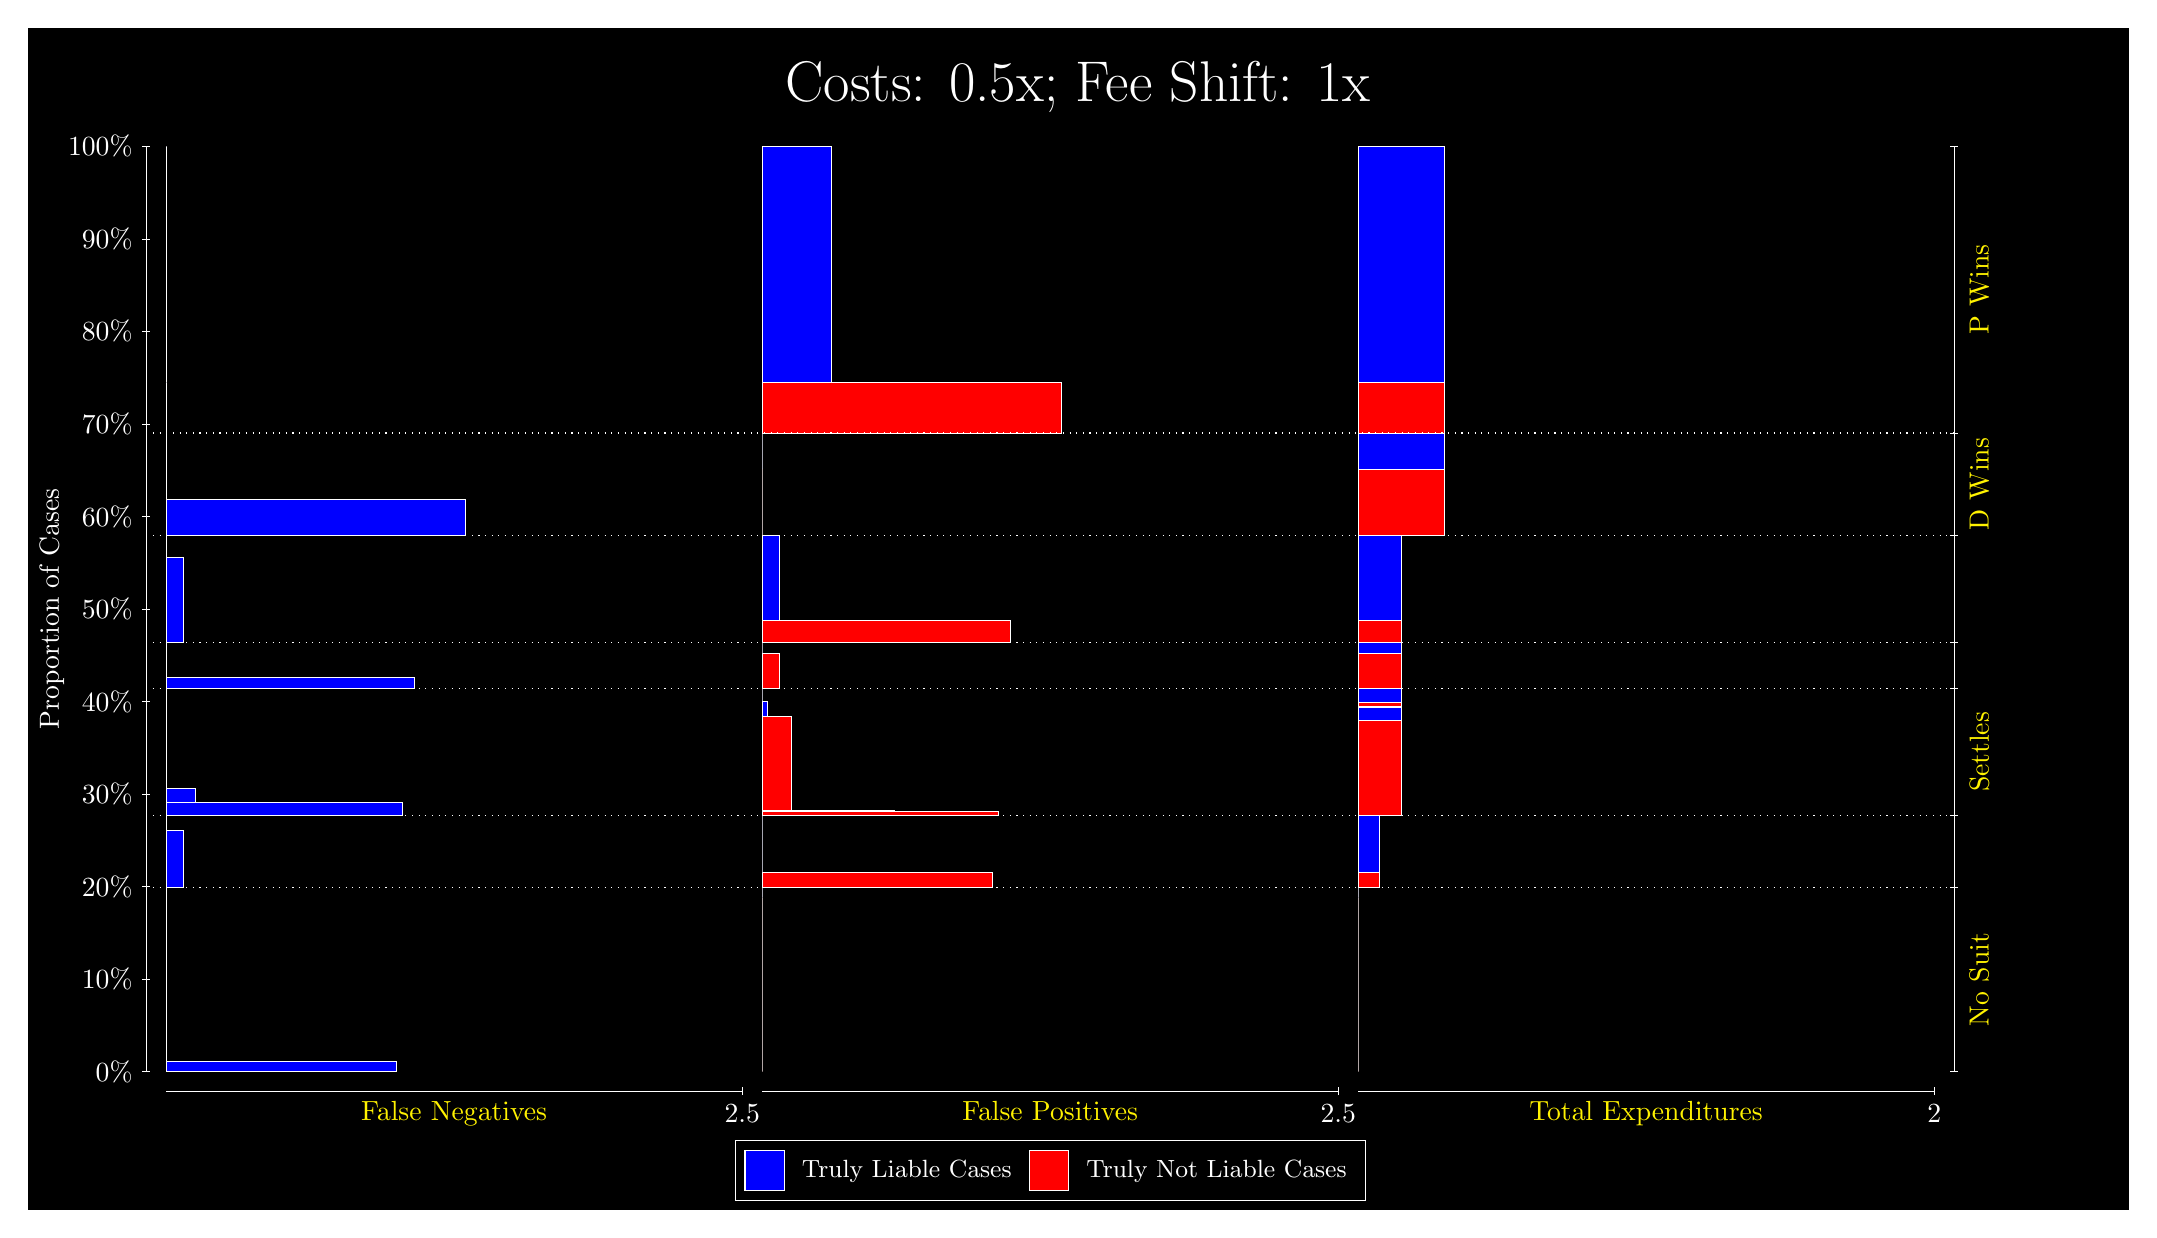
\begin{tikzpicture}
\draw[fill=black] (0,0) rectangle (26.667,15);
\draw[text=white] (0,13.5) rectangle (26.667,15) node[midway] {\huge Costs: 0.5x; Fee Shift: 1x};
\draw[white, very thin] (1.5,1.75) -- (1.5,13.5);
\node[rotate=90, text=white, anchor=center] at (0.3, 7.625) {Proportion of Cases};
\draw[white, very thin] (1.45,1.75) -- (1.55,1.75);
\node[text=white, anchor=east] at (1.45, 1.75) {0\%};
\draw[white, very thin] (1.45,2.925) -- (1.55,2.925);
\node[text=white, anchor=east] at (1.45, 2.925) {10\%};
\draw[white, very thin] (1.45,4.1) -- (1.55,4.1);
\node[text=white, anchor=east] at (1.45, 4.1) {20\%};
\draw[white, very thin] (1.45,5.275) -- (1.55,5.275);
\node[text=white, anchor=east] at (1.45, 5.275) {30\%};
\draw[white, very thin] (1.45,6.45) -- (1.55,6.45);
\node[text=white, anchor=east] at (1.45, 6.45) {40\%};
\draw[white, very thin] (1.45,7.625) -- (1.55,7.625);
\node[text=white, anchor=east] at (1.45, 7.625) {50\%};
\draw[white, very thin] (1.45,8.8) -- (1.55,8.8);
\node[text=white, anchor=east] at (1.45, 8.8) {60\%};
\draw[white, very thin] (1.45,9.975) -- (1.55,9.975);
\node[text=white, anchor=east] at (1.45, 9.975) {70\%};
\draw[white, very thin] (1.45,11.15) -- (1.55,11.15);
\node[text=white, anchor=east] at (1.45, 11.15) {80\%};
\draw[white, very thin] (1.45,12.325) -- (1.55,12.325);
\node[text=white, anchor=east] at (1.45, 12.325) {90\%};
\draw[white, very thin] (1.45,13.5) -- (1.55,13.5);
\node[text=white, anchor=east] at (1.45, 13.5) {100\%};

\draw[white, very thin] (24.457,1.75) -- (24.457,13.5);
\draw[white, very thin] (24.407,1.75) -- (24.507,1.75);
\node[anchor=west] at (24.407, 1.75) {};
\draw[white, very thin] (24.407,4.0862) -- (24.507,4.0862);
\node[anchor=west] at (24.407, 4.0862) {};
\draw[white, very thin] (24.407,5.0028) -- (24.507,5.0028);
\node[anchor=west] at (24.407, 5.0028) {};
\draw[white, very thin] (24.407,6.6163) -- (24.507,6.6163);
\node[anchor=west] at (24.407, 6.6163) {};
\draw[white, very thin] (24.407,7.2005) -- (24.507,7.2005);
\node[anchor=west] at (24.407, 7.2005) {};
\draw[white, very thin] (24.407,8.5585) -- (24.507,8.5585);
\node[anchor=west] at (24.407, 8.5585) {};
\draw[white, very thin] (24.407,9.8596) -- (24.507,9.8596);
\node[anchor=west] at (24.407, 9.8596) {};
\draw[white, very thin] (24.407,13.5) -- (24.507,13.5);
\node[anchor=west] at (24.407, 13.5) {};

\draw[white, very thin, fill=blue] (1.75,1.75) rectangle (4.6775,1.8763);
\draw[white, very thin, fill=red] (1.75,1.8763) rectangle (1.75,4.0862);
\draw[white, very thin, fill=blue] (1.75,4.0862) rectangle (1.9696,4.8103);
\draw[white, very thin, fill=red] (1.75,4.8103) rectangle (1.75,5.0028);
\draw[white, very thin, fill=blue] (1.75,5.0028) rectangle (4.7507,5.1675);
\draw[white, very thin, fill=blue] (1.75,5.1675) rectangle (3.4333,5.1698);
\draw[white, very thin, fill=blue] (1.75,5.1698) rectangle (2.1159,5.3528);
\draw[white, very thin, fill=red] (1.75,5.3528) rectangle (1.75,6.6163);
\draw[white, very thin, fill=blue] (1.75,6.6163) rectangle (4.8971,6.7563);
\draw[white, very thin, fill=red] (1.75,6.7563) rectangle (1.75,7.2005);
\draw[white, very thin, fill=blue] (1.75,7.2005) rectangle (1.9696,8.2784);
\draw[white, very thin, fill=red] (1.75,8.2784) rectangle (1.75,8.5585);
\draw[white, very thin, fill=blue] (1.75,8.5585) rectangle (5.5558,9.0142);
\draw[white, very thin, fill=red] (1.75,9.0142) rectangle (1.75,9.8596);
\draw[white, very thin, fill=red] (1.75,9.8596) rectangle (1.75,10.499);
\draw[white, very thin, fill=blue] (1.75,10.499) rectangle (1.75,13.5);
\draw[white, very thin, fill=red] (9.3189,1.75) rectangle (9.3189,3.9598);
\draw[white, very thin, fill=blue] (9.3189,3.9598) rectangle (9.3189,4.0862);
\draw[white, very thin, fill=red] (9.3189,4.0862) rectangle (12.246,4.2787);
\draw[white, very thin, fill=blue] (9.3189,4.2787) rectangle (9.3189,5.0028);
\draw[white, very thin, fill=red] (9.3189,5.0028) rectangle (12.32,5.0499);
\draw[white, very thin, fill=red] (9.3189,5.0499) rectangle (11.002,5.0627);
\draw[white, very thin, fill=red] (9.3189,5.0627) rectangle (9.6848,6.2664);
\draw[white, very thin, fill=blue] (9.3189,6.2664) rectangle (9.3921,6.4494);
\draw[white, very thin, fill=blue] (9.3189,6.4494) rectangle (9.3189,6.6163);
\draw[white, very thin, fill=red] (9.3189,6.6163) rectangle (9.5384,7.0605);
\draw[white, very thin, fill=blue] (9.3189,7.0605) rectangle (9.3189,7.2005);
\draw[white, very thin, fill=red] (9.3189,7.2005) rectangle (12.466,7.4806);
\draw[white, very thin, fill=blue] (9.3189,7.4806) rectangle (9.5384,8.5585);
\draw[white, very thin, fill=red] (9.3189,8.5585) rectangle (9.3189,9.4039);
\draw[white, very thin, fill=blue] (9.3189,9.4039) rectangle (9.3189,9.8596);
\draw[white, very thin, fill=red] (9.3189,9.8596) rectangle (13.125,10.499);
\draw[white, very thin, fill=blue] (9.3189,10.499) rectangle (10.197,13.5);
\draw[white, very thin, fill=red] (16.888,1.75) rectangle (16.888,3.9598);
\draw[white, very thin, fill=blue] (16.888,3.9598) rectangle (16.888,4.0862);
\draw[white, very thin, fill=red] (16.888,4.0862) rectangle (17.162,4.2787);
\draw[white, very thin, fill=blue] (16.888,4.2787) rectangle (17.162,5.0028);
\draw[white, very thin, fill=red] (16.888,5.0028) rectangle (17.437,6.2065);
\draw[white, very thin, fill=blue] (16.888,6.2065) rectangle (17.437,6.3712);
\draw[white, very thin, fill=red] (16.888,6.3712) rectangle (17.437,6.384);
\draw[white, very thin, fill=blue] (16.888,6.384) rectangle (17.437,6.3863);
\draw[white, very thin, fill=red] (16.888,6.3863) rectangle (17.437,6.4333);
\draw[white, very thin, fill=blue] (16.888,6.4333) rectangle (17.437,6.6163);
\draw[white, very thin, fill=red] (16.888,6.6163) rectangle (17.437,7.0605);
\draw[white, very thin, fill=blue] (16.888,7.0605) rectangle (17.437,7.2005);
\draw[white, very thin, fill=red] (16.888,7.2005) rectangle (17.437,7.4806);
\draw[white, very thin, fill=blue] (16.888,7.4806) rectangle (17.437,8.5585);
\draw[white, very thin, fill=red] (16.888,8.5585) rectangle (17.986,9.4039);
\draw[white, very thin, fill=blue] (16.888,9.4039) rectangle (17.986,9.8596);
\draw[white, very thin, fill=red] (16.888,9.8596) rectangle (17.986,10.499);
\draw[white, very thin, fill=blue] (16.888,10.499) rectangle (17.986,13.5);
\draw[white, dotted] (1.5,4.0862) -- (24.457,4.0862);
\draw[white, dotted] (1.5,5.0028) -- (24.457,5.0028);
\draw[white, dotted] (1.5,6.6163) -- (24.457,6.6163);
\draw[white, dotted] (1.5,7.2005) -- (24.457,7.2005);
\draw[white, dotted] (1.5,8.5585) -- (24.457,8.5585);
\draw[white, dotted] (1.5,9.8596) -- (24.457,9.8596);
\draw[white, very thin] (1.75,1.5) -- (9.0689,1.5);
\node[text=yellow, anchor=north] at (5.4094, 1.5) {False Negatives};
\draw[white, very thin] (9.0689,1.45) -- (9.0689,1.55);
\node[text=white, anchor=north] at (9.0689, 1.45) {2.5};

\draw[white, very thin] (9.3189,1.5) -- (16.638,1.5);
\node[text=yellow, anchor=north] at (12.978, 1.5) {False Positives};
\draw[white, very thin] (16.638,1.45) -- (16.638,1.55);
\node[text=white, anchor=north] at (16.638, 1.45) {2.5};

\draw[white, very thin] (16.888,1.5) -- (24.207,1.5);
\node[text=yellow, anchor=north] at (20.547, 1.5) {Total Expenditures};
\draw[white, very thin] (24.207,1.45) -- (24.207,1.55);
\node[text=white, anchor=north] at (24.207, 1.45) {2};

\node[text=yellow, centered, rotate=90] at (24.777, 2.9181) {No Suit};

\node[text=yellow, centered, rotate=90] at (24.777, 5.8096) {Settles};


\node[text=yellow, centered, rotate=90] at (24.777, 9.2091) {D Wins};
\node[text=yellow, centered, rotate=90] at (24.777, 11.68) {P Wins};

\draw (12.978300999999998,1.5) node[draw=none] (baseCoordinate) {};
\begin{scope}[align=center]
        \matrix[scale=0.5, draw=white, below=0.5cm of baseCoordinate, nodes={draw}, column sep=0.1cm]{
            \node[rectangle, draw, minimum width=0.5cm, minimum height=0.5cm, fill=blue] {}; &
            \node[draw=none, font=\small, text=white] (B) {Truly Liable Cases}; &
            \node[rectangle, draw, minimum width=0.5cm, minimum height=0.5cm, fill=red] {}; &
            \node[draw=none, font=\small, text=white] (B) {Truly Not Liable Cases}; \\
            };
\end{scope}

\end{tikzpicture}
\end{document}